\documentclass{llncs}
%
\usepackage[german,american]{babel}
\usepackage[latin1]{inputenc}
% \usepackage{makeidx}  % allows for indexgeneration
\usepackage{graphicx}
\usepackage{epsfig}
\usepackage{hyperref}
\usepackage{moreverb}

%
\newcommand{\todo}[1]{\emph{[ToDo: #1]}}
%
\begin{document}

\title{DBpedia: A Nucleus for a Web of Open Data}

\titlerunning{DBpedia}

\author{S\"oren Auer\inst{1,3} \and Christian Bizer\inst{2} \and Georgi Kobilarov\inst{2} \and Jens Lehmann\inst{1} \and Richard Cyganiak\inst{2} \and Zachary Ives\inst{3}}

\authorrunning{S\"oren Auer et al.}

\tocauthor{S\"oren Auer (University of Pennsylvania),
Jens Lehmann (Universit\"at Leipzig)}
%
\institute{
Universit\"at Leipzig, Department of Computer Science, Johannisgasse 26,\\
D-04103 Leipzig, Germany,\\
\email{\{auer,lehmann\}@informatik.uni-leipzig.de}
\and
Freie Universit\"at Berlin, Web-based Systems Group, Garystr. 21,\\
D-14195 Berlin, Germany,\\
\email{chris@bizer.de, georgi.kobilarov@gmx.de richard@cyganiak.de}
\and
University of Pennsylvania, Department of Computer and Information Science\\
Philadelphia, PA 19104, USA,\\
\email{auer@seas.upenn.edu, zives@cis.upenn.edu}
}

\maketitle

\begin{abstract}
DBpedia is a community effort to extract structured information from Wikipedia
and to make this information available on the Web. DBpedia allows you to ask
sophisticated queries against datasets derived from Wikipedia and to link other
datasets on the Web to Wikipedia data. We describe the extraction of the DBpedia
datasets, and how the resulting information is published on the Web for human- and
machine-consumption. We describe some emerging applications from the DBpedia community and show how website authors can facilitate DBpedia content within their sites. Finally, we present the current status of interlinking DBpedia with other open datasets on the Web and outline how DBpedia could serve as a nucleus for an emerging Web of open data.
\end{abstract}

\section{Introduction}
\label{sec:introduction}

It is now almost universally acknowledged that stitching together the
world's structured information and knowledge to answer semantically
rich queries is one of the key challenges of computer science, and one
that is likely to have tremendous impact on the world as a whole.
This has led to almost 30 years of research into information
integration~\cite{multibase,DBLP:conf/sigmod/Wiederhold93} and
ultimately to the Semantic Web and related
technologies~\cite{chatty-web,p2p-mediation,hyperion}.  Such efforts
have generally only gained traction in relatively small and
specialized domains, where a closed ontology, vocabulary, or schema
could be agreed upon.  However, the broader Semantic Web vision has
not yet been realized, and one of the biggest challenges facing such
efforts has been how to get enough ``interesting'' and broadly useful
information into the system to make it useful and accessible to a
\emph{general} audience. 
%(For instance, there is only a limited amount of RDF available, and few OWL ontologies are widely adopted.)

A challenge is that the traditional ``top-down'' model of designing an
ontology or schema \emph{before} developing the data breaks down at
the scale of the Web: both data and metadata must constantly evolve,
and they must serve many different communities.  Hence, there has been
a recent movement to build the Semantic Web grass-roots-style,
using incremental and Web 2.0-inspired collaborative
approaches~\cite{cidr-chasm,orchestra-cidr,hyperion}. % ,DBLP:journals/debu/DoanRCDLMSS06}.
Such a collaborative, grass-roots Semantic Web requires a new model of
structured information representation and management: first and
foremost, it must handle inconsistency, ambiguity, uncertainty, data
provenance~\cite{DBLP:conf/vldb/BenjellounSHW06,DBLP:conf/icdt/BunemanKT01,cui-thesis,chrisDiss},
and implicit knowledge in a uniform way.

Perhaps the most effective way of spurring synergistic research along
these directions is to provide a rich corpus of diverse data.  This
would enable researchers to develop, compare, and evaluate different
extraction, reasoning, and uncertainty management techniques, and to
deploy operational systems on the Web. 

The DBpedia project has derived such a
data corpus from the Wikipedia encyclopedia. Wikipedia is heavily visited and under constant revision
(e.g., according to alexa.com, Wikipedia was the 9th most visited
website in the third quarter of 2007).  Wikipedia editions are
available in over 250 languages, with the English one accounting for
more than 1.95 million articles.  Like many other web applications,
Wikipedia has the problem that its search capabilities are limited to
full-text search, which only allows very limited access to this
valuable knowledge base.  As has been highly publicized, Wikipedia
also exhibits many of the challenging properties of collaboratively
edited data: it has contradictory data, inconsistent taxonomical
conventions, errors, and even spam.

The DBpedia project focuses on the task of converting Wiki\-pe\-dia content into structured knowledge, such that Semantic Web
techniques can be employed against it --- asking sophisticated queries
against Wikipedia, linking it to other datasets on the Web, or creating
new applications or mashups.  We make the following contributions:

\begin{itemize}

\item We develop an information extraction framework, which converts 
Wikipedia content to RDF. The basic components form a foundation
upon which further research into information extraction, clustering,
uncertainty management, and query processing may be conducted.

\item We provide Wikipedia content as a large, multi-domain RDF dataset, which can be used in a variety of Semantic 
Web applications. The DBpedia dataset consists of 103 million RDF triples.

\item We interlink the DBpedia dataset with other open datasets. This results in a large Web of data containing altogether around 2 billion RDF triples.

\item We develop a series of interfaces and access modules, such that the dataset
can be accessed via Web services and linked to other sites.

\end{itemize}

The DBpedia datasets can be either imported into third party applications or can be accessed online using a variety of DBpedia user interfaces. Figure \ref{fig:architecture} gives an overview about the DBpedia information extraction process and shows how extracted data is published on the Web. These main DBpedia interfaces currently use Virtuoso \cite{aksw.org/cssw07/paper/5_erling.pdf} and MySQL as storage back-ends.

\begin{figure}[h]
	\centering
		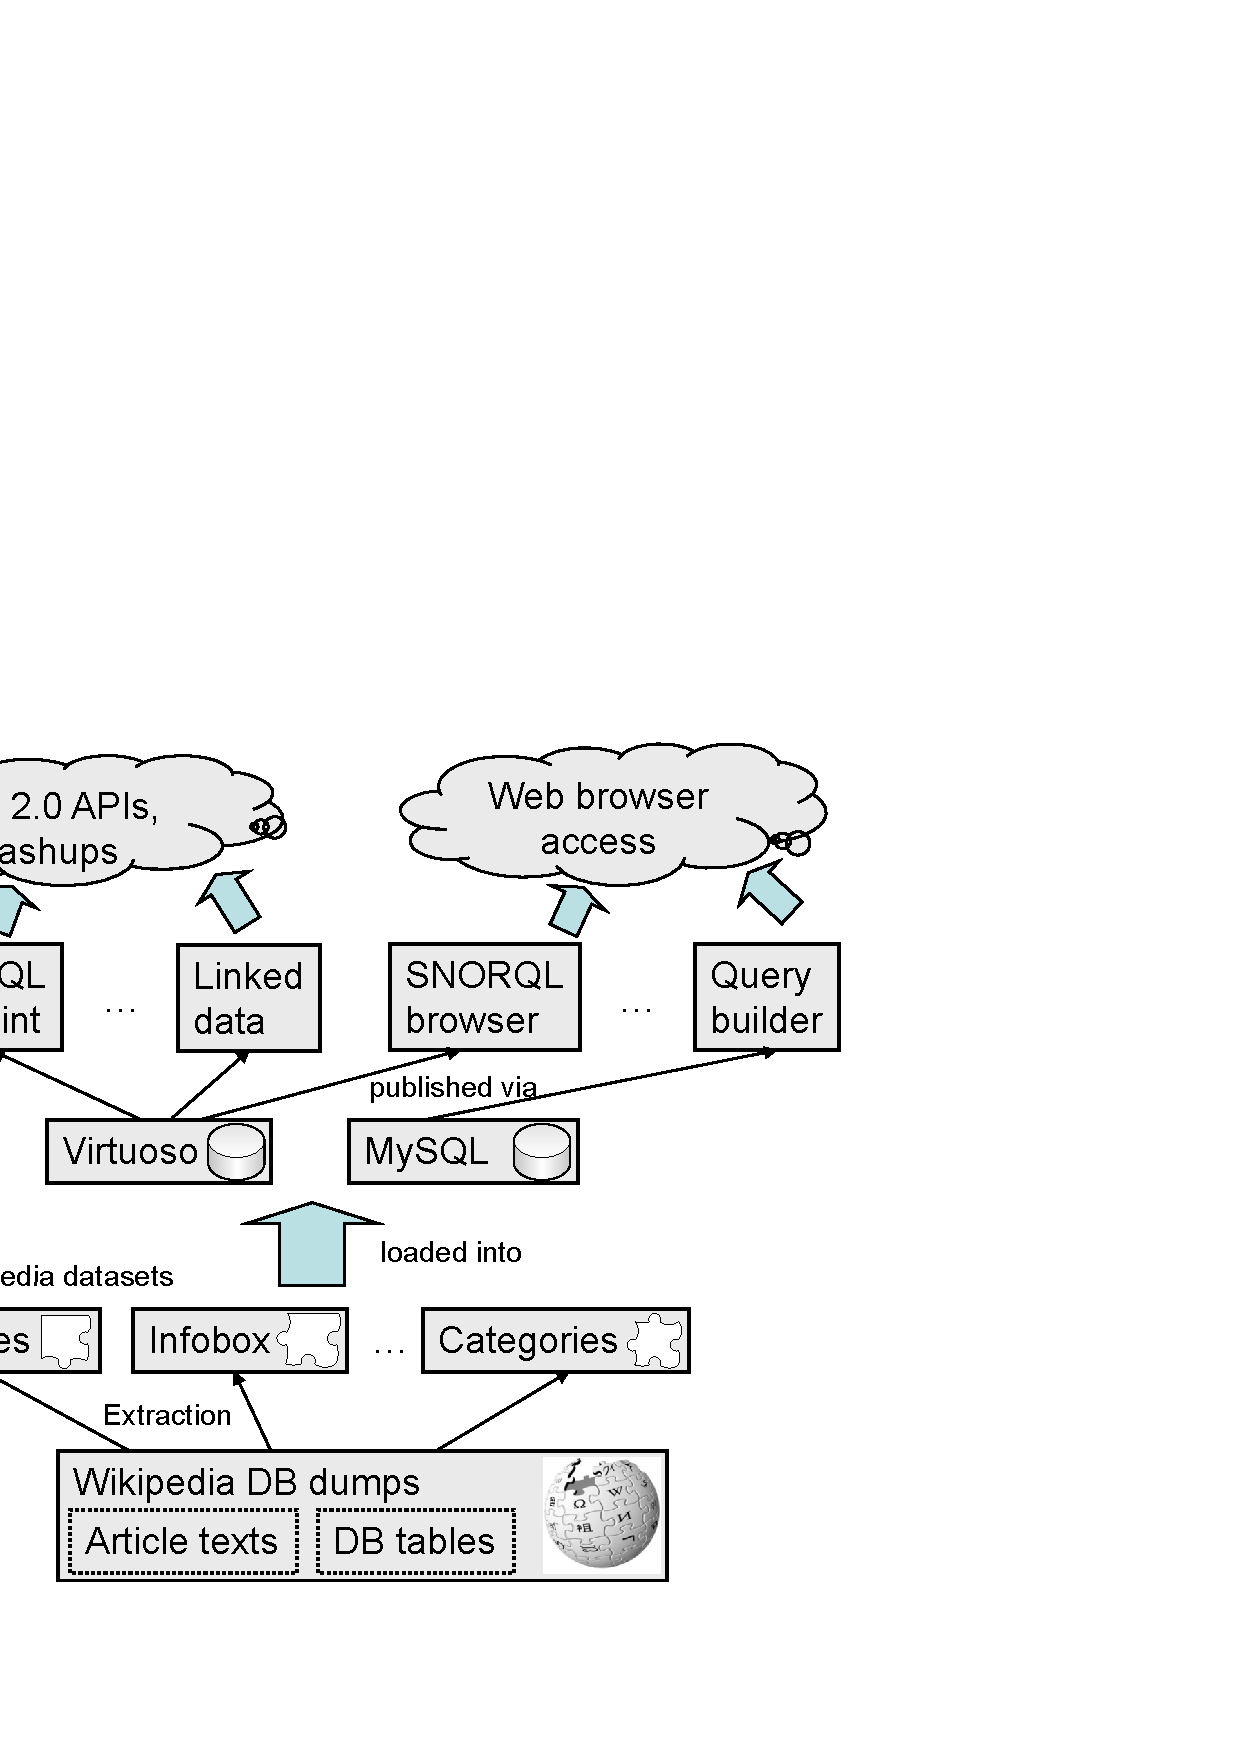
\includegraphics[width=0.6\textwidth]{architecture.pdf}
	\caption{Overview of the DBpedia components.}
	\label{fig:architecture}
\end{figure}

The paper is structured as follows: We give an overview about the DBpedia information extraction techniques in Section \ref{sec:extraction}. The resulting datasets are described in Section \ref{sec:datasets}. We exhibit methods for programmatic access to the DBpedia dataset in Section \ref{sec:access}. In Sections \ref{sec:interlinking} % and \ref{sec:integration} 
we present our vision of how the DBpedia datasets can be a nucleus for a Web of open data. We showcase several user interfaces for accessing DBpedia in Section \ref{sec:ui} and finally review related work in Section \ref{sec:related}. 

\section{Extracting Structured Information from Wikipedia}
\label{sec:extraction}

Wikipedia articles consist mostly of free text, but also contain different types of structured information, such as infobox templates, categorisation information, images, geo-coordinates, links to external Web pages and links across different language editions of Wikipedia.

Mediawiki\footnote{\url{http://www.mediawiki.org}} is the software used to run Wikipedia. Due to the nature of this Wiki system, basically all editing, linking, annotating with meta-data is done inside article texts by adding special syntactic constructs. Hence, structured information can be obtained by parsing article texts for these syntactic constructs.

Since MediaWiki exploits some of this information itself for rendering the user interface, some information is cached in relational database tables. Dumps of the crucial relational database tables (including the ones containing the article texts) for different Wikipedia language versions are published on the Web on a regular basis\footnote{\url{http://download.wikimedia.org/}}. Based on these database dumps, we currently use two different methods of extracting semantic relationships: (1) We map the relationships that are already stored in relational database tables onto RDF and (2) we extract additional information directly from the article texts and infobox templates within the articles.

\begin{figure}[tbp]
\begin{minipage}[b]{.57\linewidth} 
\centering
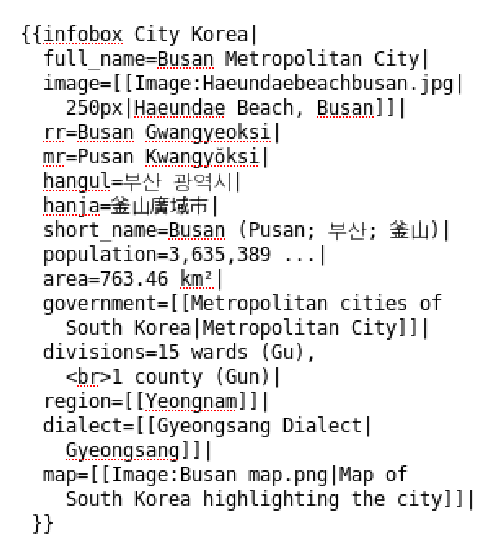
\includegraphics[width=\textwidth]{busan_infobox2}
\end{minipage}
%\hspace{.03\linewidth}
\begin{minipage}[b]{.42\linewidth}
\centering
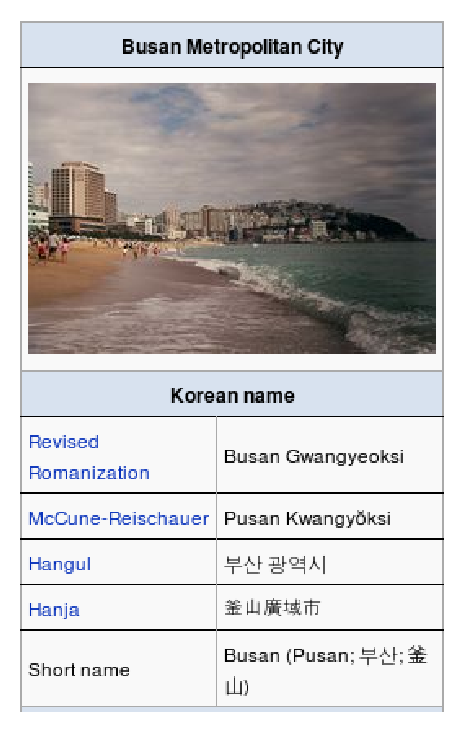
\includegraphics[width=\textwidth]{busan}
\end{minipage}
\caption{Example of a Wikipedia template and rendered output (excerpt).}
\label{fig:template}
\vspace{-5pt}
\end{figure}

We illustrate the extraction of semantics from article texts with an Wikipedia infobox template example. Figure \ref{fig:template} shows the infobox template (encoded within a Wikipedia article) and the rendered output of the South-Korean town Busan. The infobox extraction algorithm detects such templates and recognizes their structure using pattern matching techniques. It selects significant templates, which are then parsed and transformed to RDF triples. The algorithm uses post-processing techniques to increase the quality of the extraction. MediaWiki links are recognized and transformed to suitable URIs, common units are detected and transformed to data types. Furthermore, the algorithm can detect lists of objects, which are transformed to RDF lists. Details about the infobox extraction algorithm (including issues like data type recognition, cleansing heuristics and identifier generation) can be found in \cite{DBLP:conf/esws/AuerL07}. All extraction algorithms are implemented using PHP and are available under an open-source license\footnote{\url{http://sf.net/projects/dbpedia}}.

\section{The DBpedia Dataset}
\label{sec:datasets}

The DBpedia dataset currently provides information about more than 1.95 million "things", including at least 80,000 persons, 70,000 places, 35,000 music albums, 12,000 films. It contains 657,000 links to images, 1,600,000 links to relevant external web pages, 180,000 external links into other RDF datasets, 207,000 Wikipedia categories and 75,000 YAGO categories~\cite{suchanek2007WWW}. 

DBpedia concepts are described by short and long abstracts in 13 different languages. These abstracts have been extracted from the English, German, French, Spanish, Italian, Portuguese, Polish, Swedish, Dutch, Japanese, Chinese, Russian, Finnish and Norwegian versions of Wikipedia. 

Altogether the DBpedia dataset consists of around 103 million RDF triples. The dataset is provided for download as a set of smaller RDF files. Table \ref{tab:DBpediaDatasets} gives an overview over these files. 

\begin{table} [h]
\vspace{-10pt}
\begin{minipage}{\textwidth}
	\centering
		\begin{tabular}{p{2.6cm}p{8.3cm}r}
			\textbf{Dataset} & \textbf{Description} & \textbf{Triples}\\
			\hline
\textit{Articles} & Descriptions of all 1.95 million concepts within the English Wikipedia including titles, short abstracts, thumbnails and links to the corresponding articles. & 7.6M  \\
\textit{Ext. Abstracts} & Additional, extended English abstracts. & 2.1M \\
\textit{Languages} & Additional titles, short abstracts and Wikipedia article links in German, French, Spanish, Italian, Portuguese, Polish, Swedish, Dutch, Japanese, Chinese, Russian, Finnish and Norwegian. & 5.7M \\
\textit{Lang. Abstracts} & Extended abstracts in 13 languages. & 1.9M \\
\textit{Infoboxes} & Data attributes for concepts that have been extracted from Wikipedia infoboxes. & 15.5M \\
\textit{External Links} & Links to external web pages about a concept. & 1.6M \\
\textit{Article Categories} & Links from concepts to categories using SKOS. & 5.2M  \\
\textit{Categories} & Information which concept is a category and how categories are related. & 1M \\
\textit{Yago Types} & Dataset containing rdf:type Statements for all DBpedia instances using classification from YAGO~\cite{suchanek2007WWW}. & 1.9 M \\ 
\textit{Persons} & Information about 80,000 persons (date and place of birth etc.) represented using the FOAF vocabulary. & 0.5M\\
\textit{Page Links} & Internal links between DBpedia instances derived from the internal pagelinks between Wikipedia articles. & 62M \\
\textit{RDF Links} & Links between DBpedia and Geonames, US Census, Musicbrainz, Project Gutenberg, the DBLP bibliography and the RDF Book Mashup.%\footnote{\url{http://sites.wiwiss.fu-berlin.de/suhl/bizer/bookmashup/}}. 
& 180K \\
		\end{tabular}\end{minipage}
\vspace{0pt}
	\caption{The DBpedia datasets.}
	\label{tab:DBpediaDatasets}
\vspace{-15pt}
\end{table}

Some datasets (such as the \textit{Persons} or \textit{Infoboxes} datasets) are semantically rich in the sense that they contain very specific information. Others (such as the \textit{PageLinks} dataset) contain meta-data (such as links between articles) without a specific semantics. However, the latter can be beneficial, e.g. for deriving measures of closeness between concepts or relevance in search results.

%\paragraph{Resource Identification.} 
Each of the 1.95 million resources described in the DBpedia dataset is identified by a URI reference of the form \texttt{http://dbpedia.org/resource/\emph{Name}}, where \emph{Name} is taken from the URL of the source Wikipedia article, which has the form \texttt{http://en.wikipedia.org/wiki/\emph{Name}}. Thus, each resource is tied directly to an English-language Wikipedia article. This yields certain beneficial properties to DBpedia identifiers:

\begin{itemize}
\item They cover a wide range of encyclopedic topics,
\item They are defined by community consensus,
\item There are clear policies in place for their management,
\item And an extensive textual definition of the concept is available at a well-known web location (the Wikipedia page).
\end{itemize}

%DBpedia thus provides a large repository of identifiers for encyclopedic concepts, backed with relevant RDF data, for use in many RDF applications.

%\paragraph{Data quality.} <= This paragraph is outdated due to the new dataset. 
%Overall, the quality of the extracted data is surprisingly high. We evaluated a random sample of 1,000 RDF statements from the infobox extraction dataset and found only 13.3\% being inaccurately extracted. These were mainly related to properties encoding layout information, template attributes containing redundant information (thus preventing a proper data type or link recognition), several pieces of information encoded in one attribute value, and missing information (e.g. due to implicit encoding in the rendering algorithm). However, in addition to these rather technical obstacles the quality of socially generated content in general depends significantly on human factors. DBpedia currently does not contain any methods for verification that the represented information is indeed correct or about detecting missing information. However, we expect positive effects on the quality and completeness of data in Wikipedia due to the increased level of visibility (also across Wikipedia pages and information domains).

\begin{comment}
% rausgenommen weil Paper zu lang und Klassifikation noch nicht in einem benutzbaren Zustand
\paragraph{Classification of DBpedia data.} Wikipedia uses a category system to organize its articles. Some of these categories can be interpreted as RDF-Schema classes. The articles in such categories can then often be seen as instances of classes and subcategories are often subclasses. Unfortunately, the transition of the Wikipedia category hierarchy to a class hierarchy is not straightforward. Some categories serve only administrative purposes, others are more a "related-to" connection than an actual subsumption relation. The YAGO project~\cite{suchanek2007WWW} tries to resolve this issue by linking Wikipedia leaf categories to WordNet concepts. However, there is still a need for a class hierarchy which is closer to the Wikipedia category system. Such a class hierarchy will increase the quality of the extracted data and can be used e.g.~for improving semantic search engines. We have identified patterns for detecting classes and their relations in the Wikipedia category system and will use this approach to extract a further classification dataset. This work still requires an amount of manual effort to improve its quality and is an ongoing process. 
\end{comment}

\section{Accessing the DBpedia Dataset on the Web}
\label{sec:access}

We provide three access mechanisms to the DBpedia dataset: Linked Data, the SPARQL protocol, and downloadable RDF dumps. Royalty-free access to these interfaces is granted under the terms of the GNU Free Documentation License.

\paragraph{Linked Data.} Linked Data is a method of publishing RDF data on the Web that relies on \texttt{http://} URIs as resource identifiers and the HTTP protocol to retrieve resource descriptions~\cite{linkedData,linkedDataHowto}. The URIs are configured to return meaningful information about the resource---typically, an RDF description containing everything that is known about it. Such a description usually mentions related resources by URI, which in turn can be accessed to yield their descriptions. This forms a dense mesh of web-accessible resource descriptions that can span server and organization boundaries. DBpedia resource identifiers, such as \url{http://dbpedia.org/resource/Busan}, are set up to return RDF descriptions when accessed by Semantic Web agents, and a simple HTML view of the same information to traditional web browsers (see Figure \ref{fig:BusanAsHTML}). HTTP content negotiation is used to deliver the appropriate format. 

Web agents that can access Linked Data include: 1. Semantic Web browsers like Disco\footnote{\url{http://sites.wiwiss.fu-berlin.de/suhl/bizer/ng4j/disco/}}, Tabulator\cite{tabulator} (see Figure \ref{fig:BusanInTabulator}), or the OpenLink Data Web Browser\footnote{\url{http://demo.openlinksw.com/DAV/JS/rdfbrowser/index.html}}; 2. Semantic Web crawlers like SWSE\footnote{\url{http://swse.org}} and Swoogle\footnote{\url{http://swoogle.umbc.edu/}};
3. Semantic Web query agents like the Semantic Web Client Library\footnote{\url{http://sites.wiwiss.fu-berlin.de/suhl/bizer/ng4j/semwebclient/}} and the SemWeb client for SWI prolog\footnote{\url{http://moustaki.org/swic/}}.

\begin{figure}[h]
\vspace{-15pt}
	\centering
		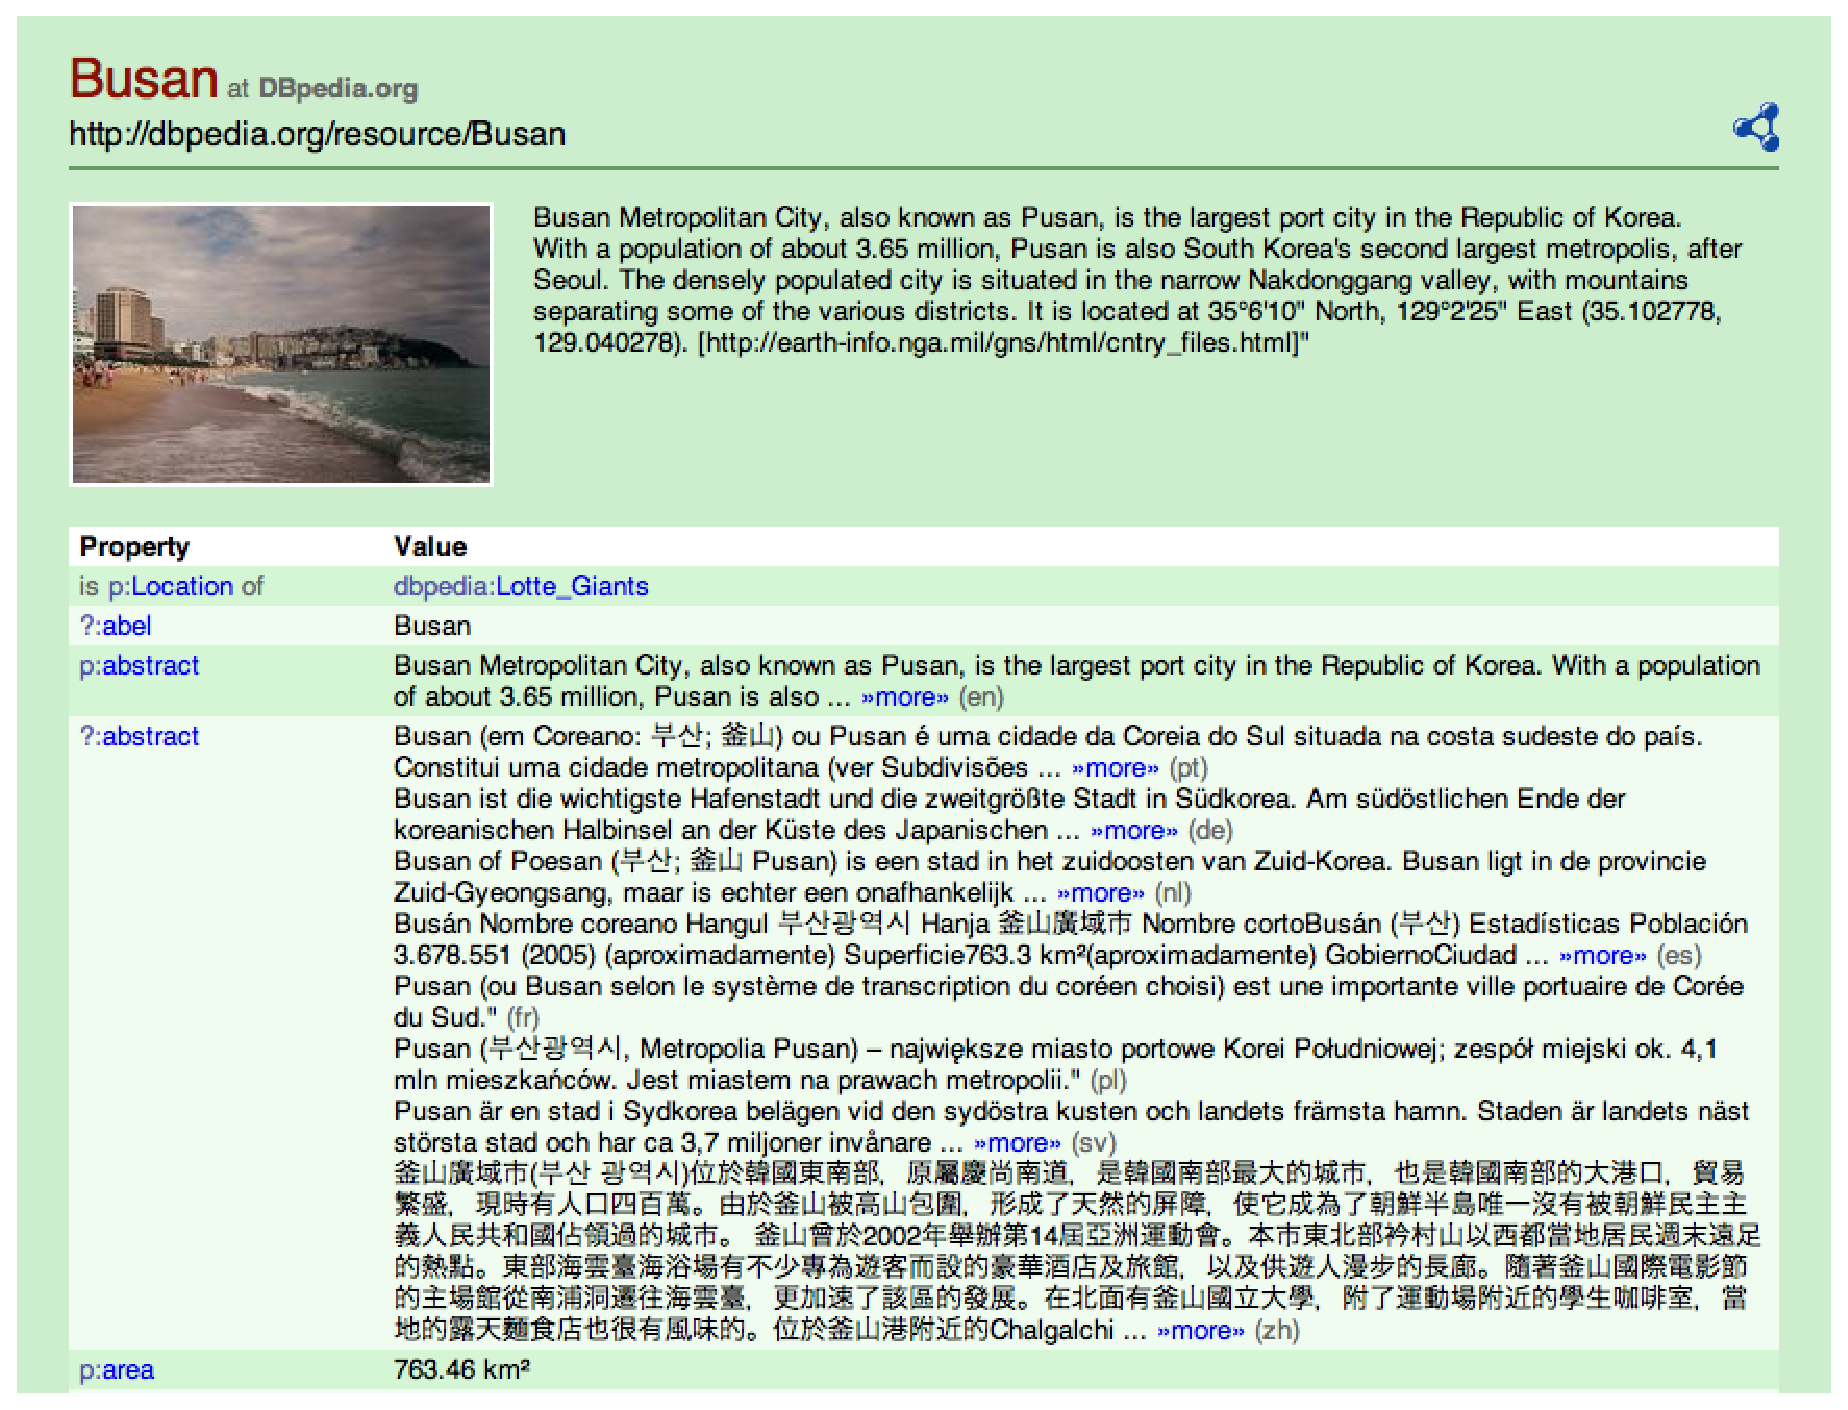
\includegraphics[width=0.49\textwidth]{busan_resource_html}
		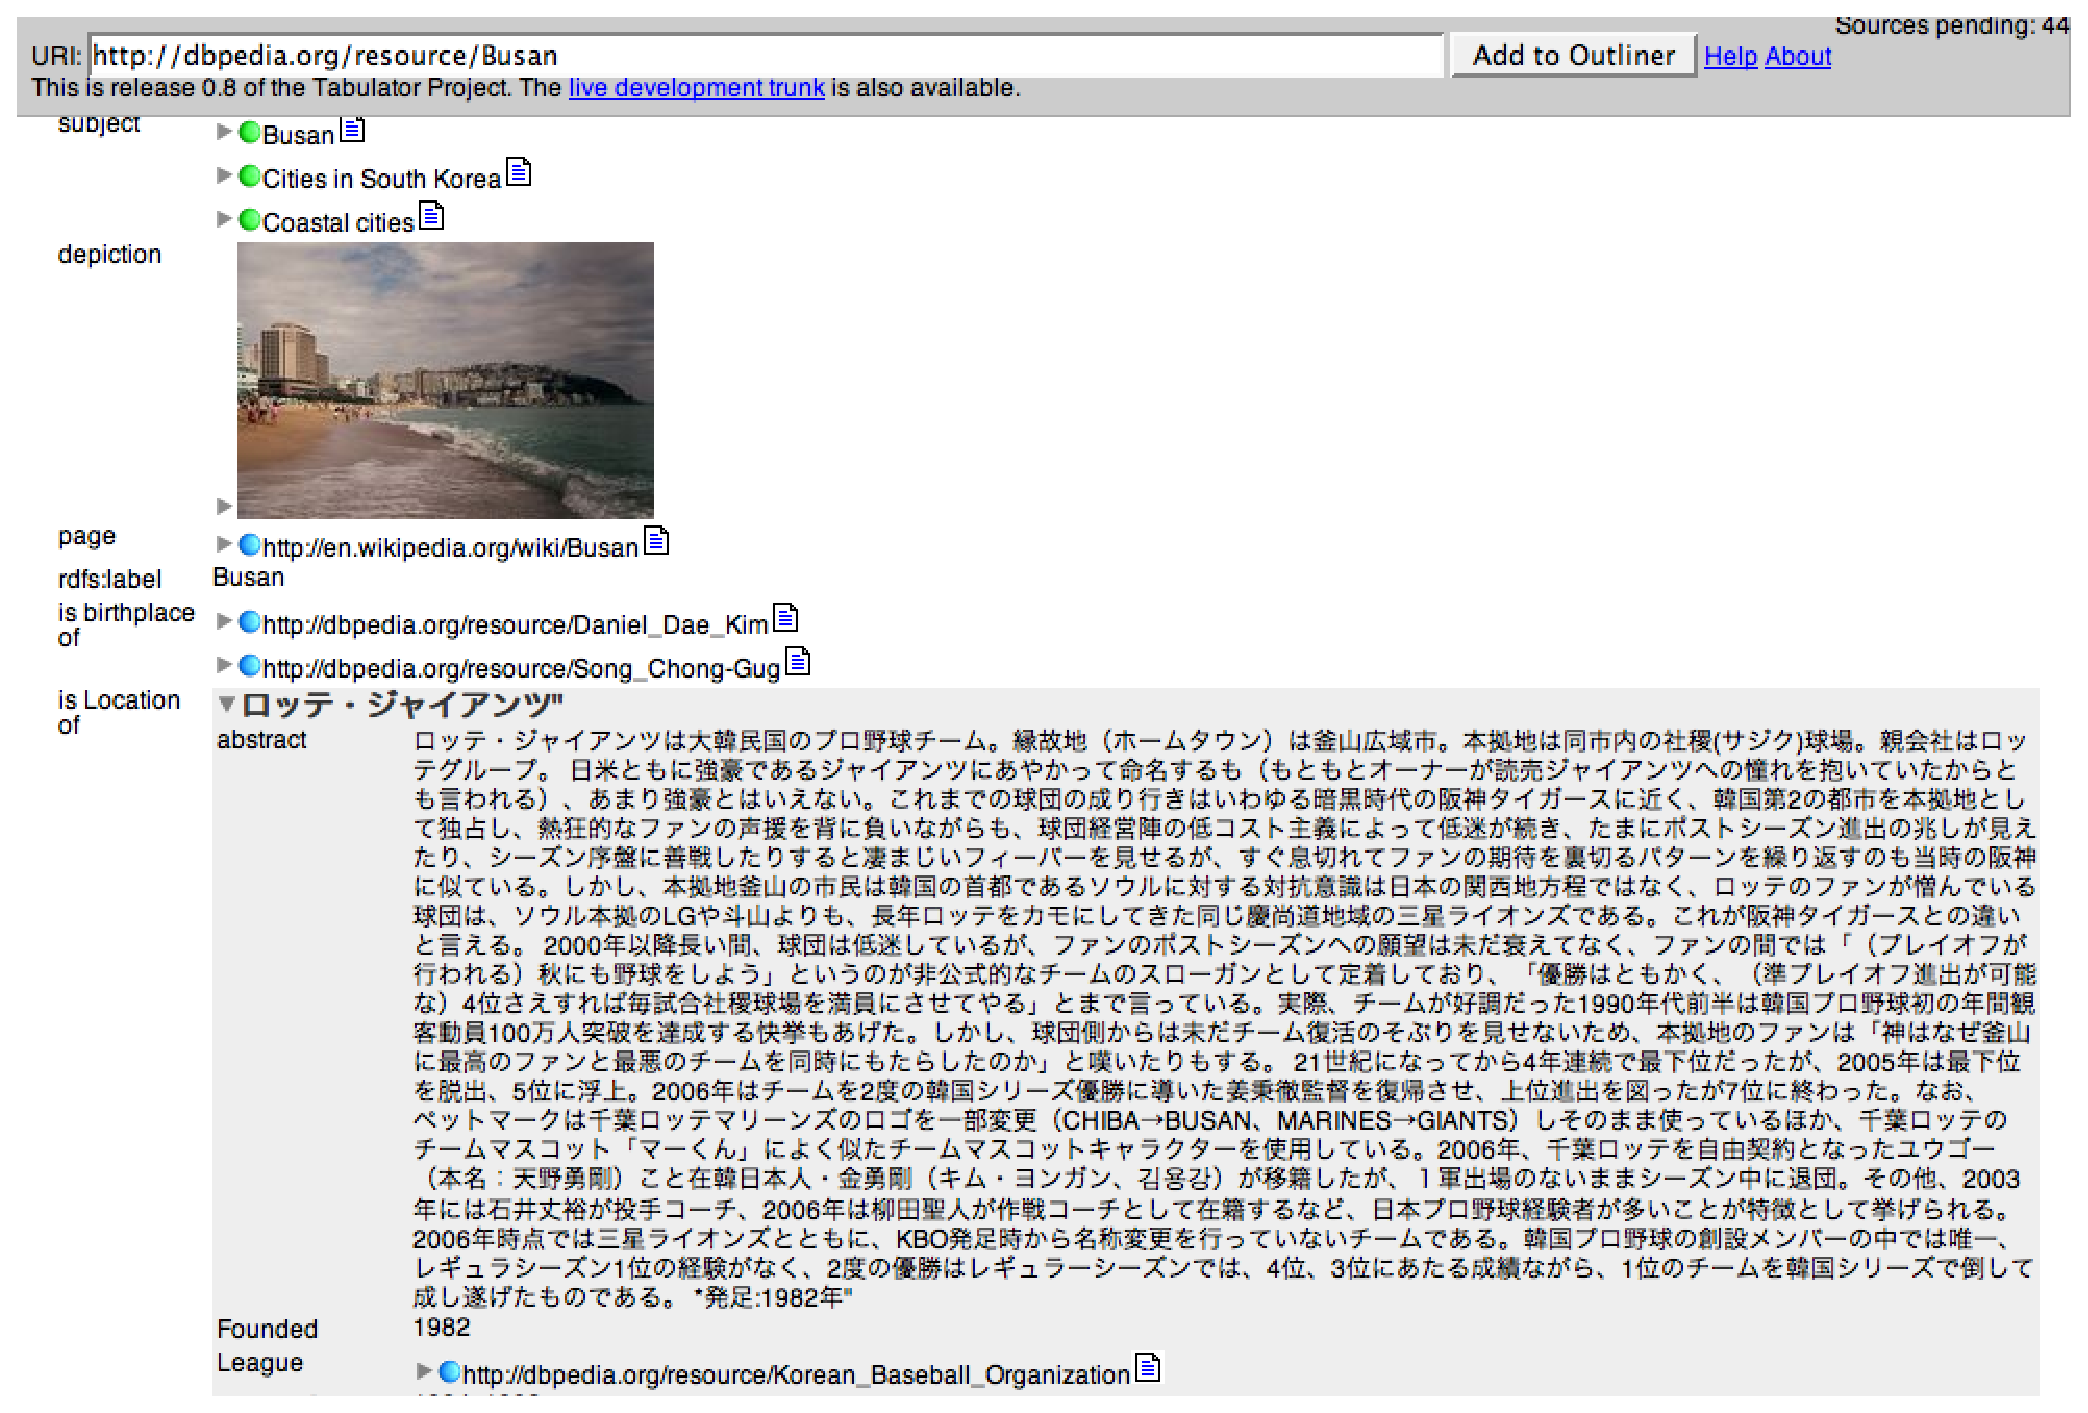
\includegraphics[width=0.49\textwidth]{busan_tabulator}
	\caption{\url{http://dbpedia.org/resource/Busan} viewed in a web browser (left) and in Tabulator (right).}
	\label{fig:BusanAsHTML}
	\label{fig:BusanInTabulator}
\vspace{-15pt}	
\end{figure}

\paragraph{SPARQL Endpoint.} We provide a SPARQL endpoint for querying the DBpedia dataset. Client applications can send queries over the SPARQL protocol to this endpoint at \url{http://dbpedia.org/sparql}. This interface is appropriate when the client application developer knows in advance exactly what information is needed. In addition to standard SPARQL, the endpoint supports several extensions of the query language that have proved useful for developing  user interfaces: full text search over selected RDF predicates, and aggregate functions, notably \texttt{COUNT}. To protect the service from overload, limits on query cost and result size are in place. For example, a query that asks for the store's entire contents is rejected as too costly. \texttt{SELECT} results are truncated at 1000 rows. The SPARQL endpoint is hosted using Virtuoso Universal Server\footnote{\url{http://virtuoso.openlinksw.com}}.

\paragraph{RDF Dumps.} N-Triple serializations of the datasets are available for download at the DBpedia website and can be used by sites that are interested in larger parts of the dataset. 


\section{Interlinking DBpedia with other Open Datasets}
\label{sec:interlinking}

In order to enable DBpedia users to discover further information, the DBpedia dataset is interlinked with various other data sources on the Web using RDF links. RDF links enable web surfers to navigate from data within one data source to related data within other sources using a Semantic Web browser. RDF links can also be followed by the crawlers of Semantic Web search engines, which may provide sophisticated search and query capabilities over crawled data. 

The DBpedia interlinking effort is part of the Linking Open Data community project\footnote{\url{http://esw.w3.org/topic/SweoIG/TaskForces/CommunityProjects/LinkingOpenData}} of the W3C Semantic Web Education and Outreach (SWEO) interest group. This community project is committed to make massive datasets and ontologies, such as the US Census, Geonames, MusicBrainz, the DBLP bibliography, WordNet, Cyc and many others, interoperable on the Semantic Web. DBpedia, with its broad topic coverage, intersects with practically all these datasets and therefore makes an excellent ``linking hub'' for such efforts.

Figure \ref{fig:lod-datasets} gives an overview about the datasets that are currently interlinked with DBpedia. Altogether this Web-of-Data amounts to approximately 2 billion RDF triples. Using these RDF links, surfers can for instance navigate from a computer scientist in DBpedia to her publications in the DBLP database, from a DBpedia
book to reviews and sales offers for this book provided by the RDF Book Mashup, or from a band in DBpedia to a list of their songs provided by Musicbrainz or dbtune.

\begin{figure}[h]
	\centering
		\includegraphics[width=0.85\textwidth]{lod-datasets.png}
	\caption{Datsets that are interlinked with DBpedia.}
	\label{fig:lod-datasets}
\end{figure}

The example RDF link shown below connects the DBpedia URI identifying Busan with further data about the city provided by Geonames: 

\begin{verbatim}
<http://dbpedia.org/resource/Busan>
    owl:sameAs <http://sws.geonames.org/1838524/> .
\end{verbatim}

Agents can follow this link, retrieve RDF from the Geonames URI, and thereby get hold of additional information about Busan as published by the Geonames server, which again contains further links deeper into the Geonames data. DBpedia URIs can also be used to express personal interests, places of residence, and similar facts within personal FOAF profiles:

\begin{verbatim}
<http://richard.cyganiak.de/foaf.rdf#cygri>
    foaf:topic_interest <http://dbpedia.org/resource/Semantic_Web> ;
    foaf:based_near <http://dbpedia.org/resource/Berlin> .
\end{verbatim}

Another use case is categorization of blog posts, news stories and other documents. The advantage of this approach is that all DBpedia URIs are backed with data and thus allow clients to retrieve more information about a topic:

\begin{verbatim}
<http://news.cnn.com/item1143>
    dc:subject <http://dbpedia.org/resource/Iraq_War> .
\end{verbatim}

%The Linked Data interface becomes especially pervasive in conjunction with these links. If the sites at both ends of such RDF statements supports the Linked Data paradigm, then the statement becomes a \emph{cross-site RDF link}.

%For example, DBpedia's description of Busan contains an \texttt{owl:sameAs} link to the same city in the Geonames dataset. 

\begin{comment}
\section{Light-weight information and application integration}
\label{sec:integration}

\todo{Der Rest des Papers praesentiert mehr oder weniger abgeschlossene Arbeit, das hier ist zwar interessant, aber hochspekulativ. Trotz der Beteuerung dass sich der Ansatz von Fenselschem SWS unterscheidet, wird mir auf so geringem Raum nicht klar worin der Unterschied besteht. Ich bin fuer streichen. Oder nach "Future Work" verfrachten, dabei kuerzen (REST vs. SOAP Debatten haben mit DBpedia nichts zu tun, hochspezifische aber nicht erklaerte Verweise auf index.html, "mappable to SOAP" etc. raus). Allgemein finde ich den zweiten und letzten Absatz gut, den Rest nicht passend fuer eine Beschreibung von DBpedia. Input/Output-Alignment koennte man alternativ auch als weiteres Beispiel in der Linking-Sektion erwaehnen. --Richard} 
\todo{Da das Paper zur Zeit zu lang ist, f�nde auch ich es gut, wenn wir diese Ideen in ein zuk�nftiges Paper verlagern w�rden, wo wir sie auch ausf�hrlicher erkl�ren k�nnen. Aber das ist ganz S�ren's Entscheidung. -- Chris}

In addition to establish simple links between data sources (as explained in the last Section), the ultimate goal of DBpedia is to contribute to a tight information and application integration on the Web. This is very related to the Web Services and Semantic Web Services initiatives. However, the understanding of Web Services within the research community (solely focusing on SOAP, WSDL, UDDI) meanwhile slightly differs from the Web Services actually deployed in a global scale. These are light-weight Web-API's, which can be accessed following the AJAX and JSON, REST paradigms. The website Programmableweb.com for example lists over 408 public and globally accessible information sources and web accessible applications and new ones are added daily.

We see DBpedia at the core of achieving a semantic integration of these light-weight Web services for two reasons. First, DBpedia provides huge multi-domain ontology, which can effectively used to align inputs and output definitions. Second, DBpedia itself provides an enormous knowledge source for the generation of a multiplicity of specialized light-weight information sources. What are the steps required to achieve this vision:

%Solution: Develop a (formal) model and Web application scenario which will enable semi-automatic integration, combination, aggregation (orchestration?) of such light-weight distributed data source.

\begin{itemize}
	\item Enable self-description of data and information sources -- such as the \verb|index.html| page for a website on a web-server. A special RDF vocabulary could serve this purpose. For the sake of simplicity, this vocabulary should be easily mappable into JSON.
	\item Allow server side views in the fashion of stored procedures or prepared statements. Such server side views can be simple, parametrized SPARQL\cite{sparql} queries with placeholders.
	\item Parameters (i.e. inputs) and return values (i.e. outputs) of such server provided views should be described semantically. For example, RDF class identifiers (URIs) can be used for annotating inputs and outputs.
\end{itemize}

Combined, this will enable end-user driven web-scale data integration in the way that information sources can be (semi-automatically) combined by aligning outputs of one information source to the inputs of another. The creation of `semantic Mashups' based on these self-describing information sources will not require any programming.
\end{comment}

\section{User Interfaces}
\label{sec:ui}

User interfaces for DBpedia can range from a simple table within a classic web page, over browsing interfaces to different types of query interfaces. This section gives an overview about the different user interfaces that have been implemented so far.

%Hence, within the DBpedia project we aim to provide a number of different query and browse facilities for exploring the DBpedia datasets.

\subsection{Simple Integration of DBpedia Data into Web Pages}

DBpedia is a valuable source of general-purpose data that can be used within web pages. Therefore, if you want a table containing German state capitals, African musicians, Amiga computer games or whatever on your website, you can generate this table using a SPARQL query against the DBpedia endpoint. Wikipedia is kept up-to-date by a large community and a nice feature of such tables is that they will also stay up-to-date as Wikipedia, and thus also DBpedia, changes. Such tables can either be implemented using Javascript on the client or with a scripting language like PHP on the server. Two examples of Javascript generated tables are found on the DBpedia website\footnote{\url{http://dbpedia.org}}.

\subsection{Search DBpedia.org}

\emph{Search DBpedia.org} is a sample application that allows users to explore the DBpedia dataset together with information from interlinked datasets such as Geonames, the RDF Book Mashup or the DBLP bibliography. In contrast to the keyword-based full-text search commonly found on the Web, search over structured data offers the opportunity to make productive use of the relations in the data, enabling stepwise narrowing of search results in different dimensions. This adds a browsing component to the search task and may reduce the common ``keyword-hit-or-not-hit'' problem.

A {\em Search DBpedia.org} session starts with a keyword search. A first set of results is computed by direct keyword matches. Related matches are added, using the relations between entities up to a depth of two nodes. Thus, a search for the keyword ``Scorsese'' will include the director Martin Scorsese, as well as all of his films, and the actors of these films.

The next step is result ranking. Our experiments showed that important articles receive more incoming page links from other articles. We use a combination of incoming link count, relevance of the link's source, and relation depth to calculate a relevance ranking.

After entering a search term, the user is presented with a list of ranked results, and with a tag cloud built from the classes found in the results, using a combination of the DBpedia and YAGO~\cite{suchanek2007WWW} classifications. Each class weight is calculated from the sum of associated result weights and the frequency of occurrence. The tag cloud enables the user to narrow the results to a specific type of entities, such as ``Actor'', even though a simple keyword search may not have brought up any actors. 

When a resource from the results is selected, the user is presented with a detailed view of all data that is known about the resource. Label, image and description are shown on top. Single-valued and multi-valued properties are shown separately. Data from interlinked datasets is automatically retrieved by following RDF links within the dataset and retrieved data from interlinked datasets is shown together with the DBpedia data.

\begin{figure}
\begin{minipage}[b]{.45\linewidth} 
	\centering
		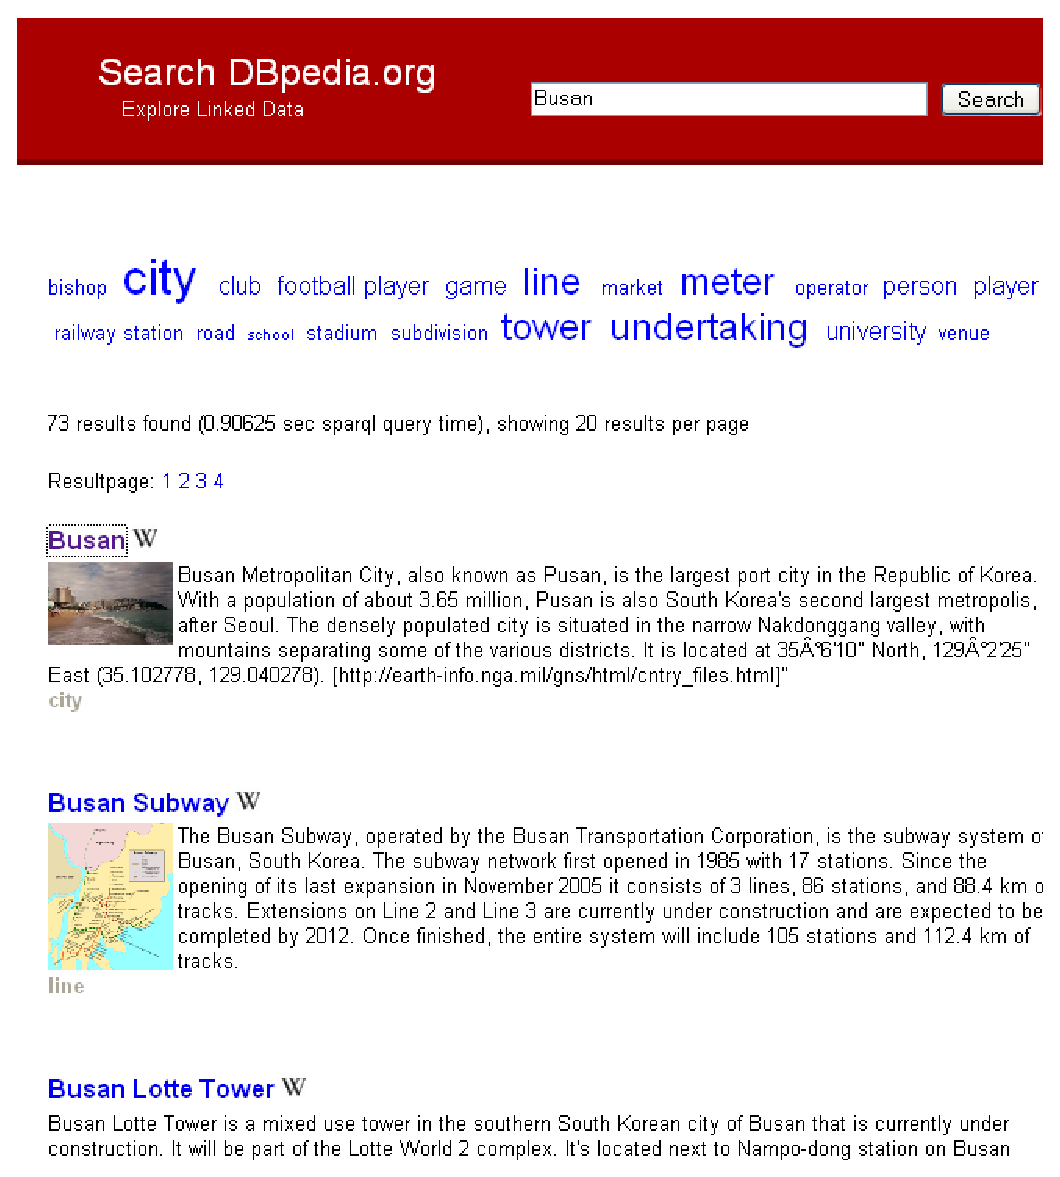
\includegraphics[width=\textwidth]{busan_search}
%	\caption{Search Results for Busan}
%	\label{fig:BusanSearch}
%\end{figure}
%\begin{figure}[h]
\end{minipage}
\hspace{3pt}
\begin{minipage}[b]{.55\linewidth} 
	\centering
	\includegraphics[width=\textwidth]{busan_search_details}
	\vspace{2pt}
%	\caption{Details View for Busan}
%	\label{fig:BusanSearchDetails}
\end{minipage}
\caption{Search results and details view for Busan.}
\label{fig:BusanSearch}
\end{figure}

\subsection{Querying DBpedia Data}

Compared to most of the other Semantic Web knowledge bases currently available, for the RDF extracted from Wikipedia we have to deal with a different type of knowledge structure \--- we have a very large information schema and a considerable amount of data adhering to this schema. Existing tools unfortunately mostly focus on either one of both parts of a knowledge base being large, schema \textit{or} data.

If we have a large data set and large data schema, elaborated RDF stores with integrated query engines alone are not very helpful. Due to the large data schema, users can hardly know which properties and identifiers are used in the knowledge base and hence can be used for querying. Consequently, users have to be guided when building queries and reasonable alternatives should be suggested.

We specifically developed a graph pattern builder for querying the extracted Wikipedia content. Users query the knowledge base by means of a graph pattern consisting of multiple triple patterns. For each triple pattern three form fields capture variables, identifiers or filters for subject, predicate and object of a triple. While users type identifier names into one of the form fields, a look-ahead search proposes suitable options. These are obtained not just by looking for matching identifiers but by executing the currently built query using a variable for the currently edited identifier and filtering the results returned for this variable for matches starting with the search string the user supplied. This method ensures, that the identifier proposed is really used in conjunction with the graph pattern under construction and that the query actually returns results. In addition, the identifier search results are ordered by usage number, showing commonly used identifiers first. All this is executed in the background, using the Web 2.0 AJAX technology and hence completely transparent for the user. Figure \ref{fig:querybuilder} shows a screenshot of the graph pattern builder.

\begin{figure}[htbp]
	\centering
		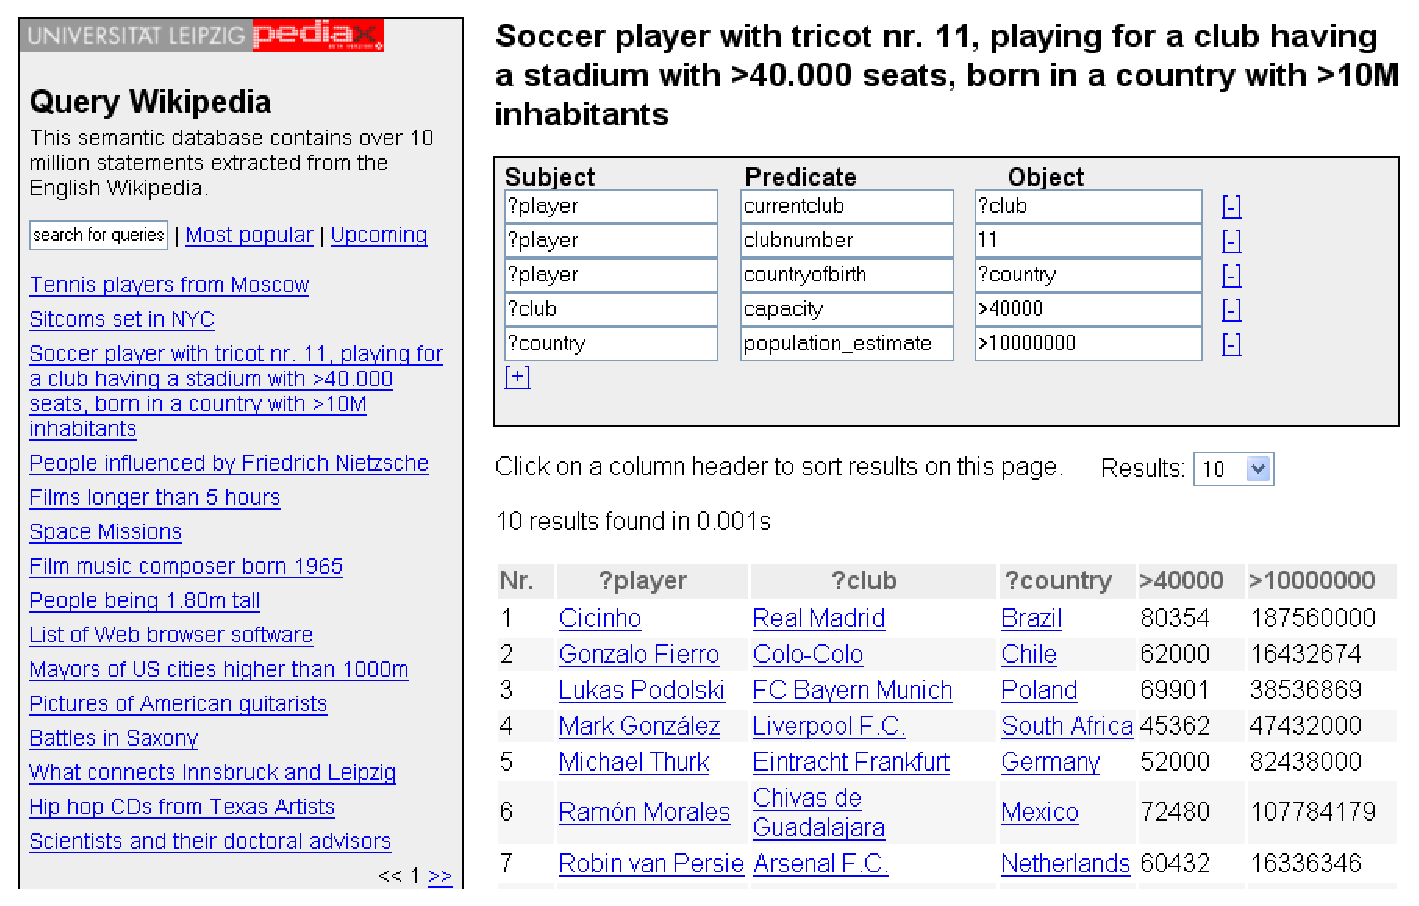
\includegraphics[width=0.80\columnwidth]{querybuilder}
	\caption{Form based query builder.}
	\label{fig:querybuilder}
\end{figure}

%Talk about SNORQL query explorer.

%Talk about Virtuoso SPARQL query builder.

% erstmal rauslassen (wird noch entwickelt)
\begin{comment}
\subsubsection*{DBpedia Object Connector}

\emph{[The DBpedia object connector is currently under construction. (Jens)]}
The DBpedia instance data can be seen as a huge RDF graph, where objects are connected by properties. An interesting application of our DBpedia data set is to answer the question what two objects have in common. This question can be answered by computing the shortest path between two objects in the DBpedia infobox RDF graph. In our search for efficient solutions for this problem, we found interesting structural properties of Wikipedia: The RDF graph cannot be easily decomposed in subgraphs, i.e.~a large fraction of the articles belong to the same subgraph. This hold true even if we remove all category connections (including articles describing categories). This indicates that Wikipedia infoboxes are deeply interlinked -- often across several domains. The connections between different objects are not always obvious. In fact, the shortest path between two objects can have a length of up to approximately ... . The DBpedia object connector can reveal interesting and often surprising connections, which are unlikely to be found by any other application. \todo{show a screenshot with an interesting example; hopefully the data connector will be finished in time (Jens)}
\end{comment}

\subsection{Third Party User Interfaces}

The DBpedia project aims at providing a hotbed for applications and mashups based on information from Wikipedia. Although DBpedia was just recently launched, there is already a number of third party applications using the dataset. Examples include:

\begin{itemize}
\item A SemanticMediaWiki~\cite{wikipediaandsw,semwiki}  installation run by the University of Karlsruhe, which has imported the DBpedia dataset together with the English edition of Wikipedia.
\item WikiStory (see Figure \ref{fig:wikistory}) which enables users to browse Wikipedia articles about people on a large timeline.
\item The Objectsheet JavaScript visual data environment,%\footnote{\url{http://www.richk.net/os/doc/what.html}},
which allows spreadsheet calculations based on DBpedia data\footnote{\url{http://richk.net/objectsheet/osc.html?file=sparql_query1.os}}.
\end{itemize}


\begin{figure}
	\centering
		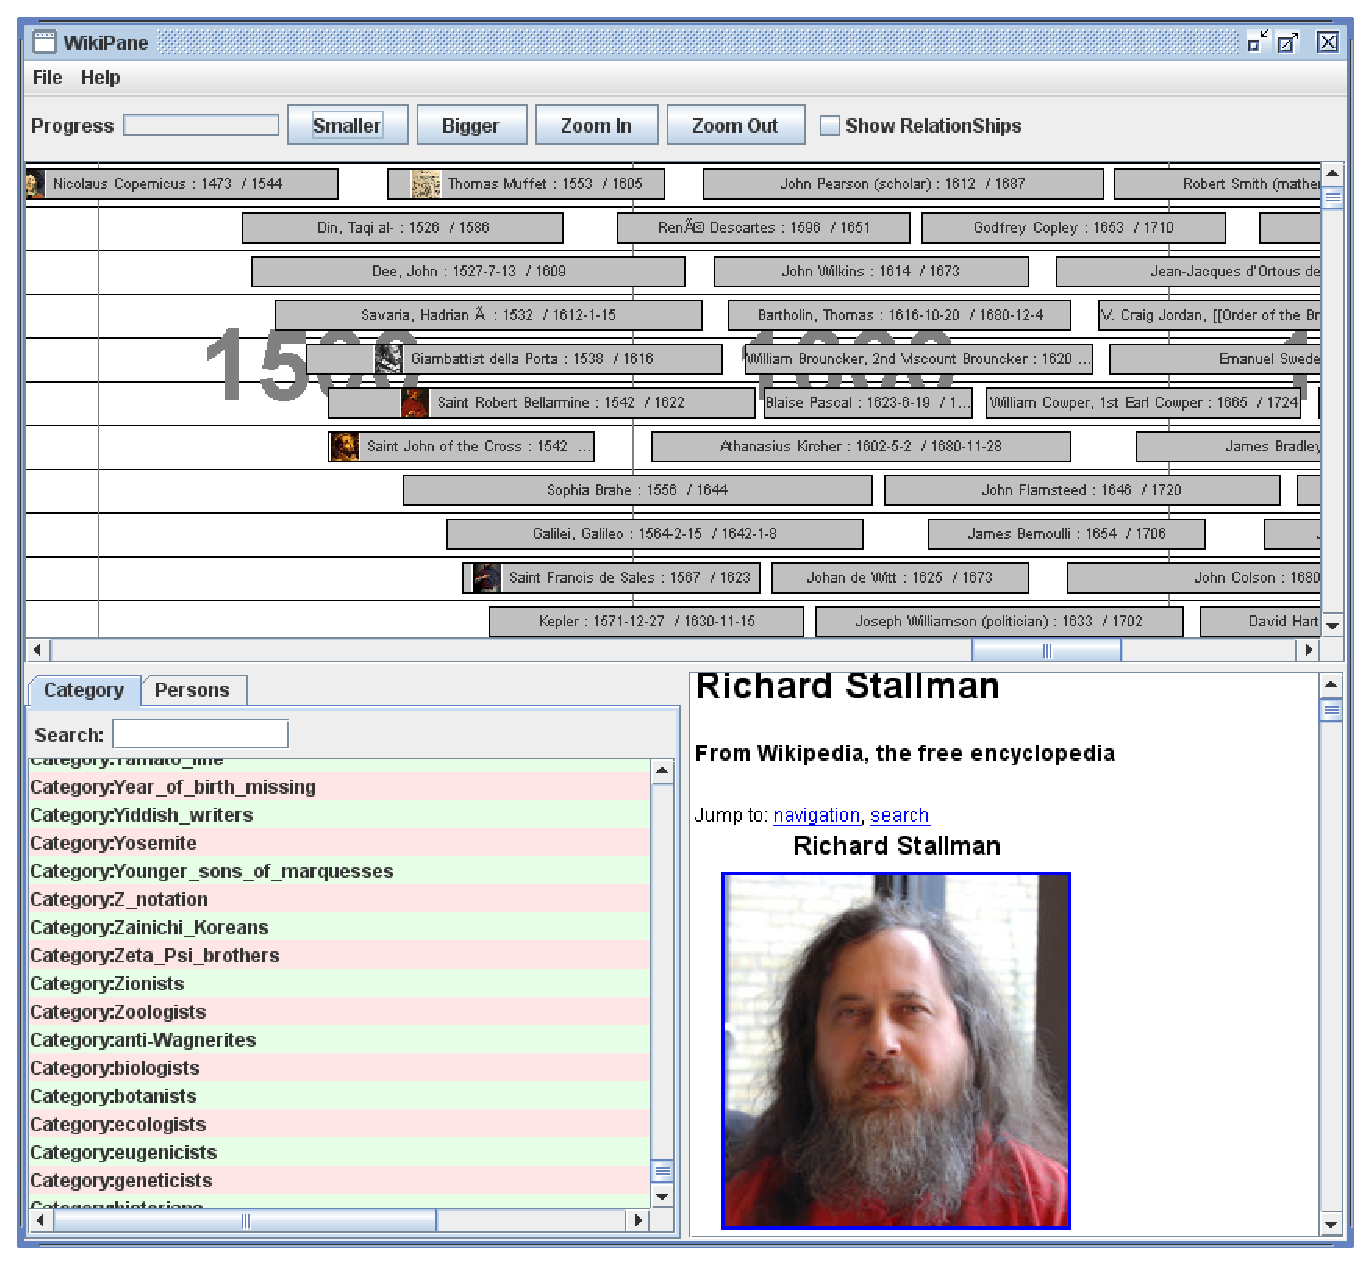
\includegraphics[width=0.50\columnwidth]{wikistory}
	\caption{WikiStory allows timeline browsing of biographies in Wikipedia.}
	\label{fig:wikistory}
\end{figure}

\section{Related Work}
\label{sec:related}

A second project that also works on extracting structured information from Wikipedia is the YAGO project~\cite{suchanek2007WWW}. YAGO extracts only 14 relationship types, such as \textit{subClassOf}, \textit{type}, \textit{familyNameOf}, \textit{locatedIn} from different sources of information in Wikipedia. One source is the Wikipedia category system (for \textit{subClassOf, locatedIn, diedInYear, bornInYear}), and another one are Wikipedia redirects. YAGO does not perform an infobox extraction as in our approach. For determining (sub-)class relationships, YAGO does not use the full Wikipedia category hierarchy, but links leaf categories to the WordNet hierarchy.

The Semantic MediaWiki project~\cite{wikipediaandsw,semwiki} also aims at enabling the reuse of information within Wikis as well as at enhancing search and browse facilities. Semantic MediaWiki is an extension of the MediaWiki software, which allows you to add structured data into Wikis using a specific syntax. Ultimately, the DBpedia and Semantic MediaWiki have similar goals. Both want to deliver the benefits of structured information in Wikipedia to the users, but use different approaches to achieve this aim. Semantic MediaWiki requires authors to deal with a new syntax and covering all structured information within Wikipedia would require to convert all information into this syntax.  DBpedia exploits the structure that already exists within Wikipedia and hence does not require deep technical or methodological changes. However, DBpedia is not as tightly integrated into Wikipedia as is planned for Semantic MediaWiki and thus is limited in constraining Wikipedia authors towards syntactical and structural consistency and homogeneity.
%Therefore, the approach does not require changes from Wikipedia authors and can be employed against the complete content of Wikipedia.

Another interesting approach is followed by Freebase\footnote{\url{http://www.freebase.com}}. The project aims at building a huge online database which users can edit in a similar fashion as they edit Wikipedia articles today. The DBpedia community cooperates with Metaweb and we will interlink data from both sources once Freebase is public.

% Find the other papers on Wikipedia info extraction and talk about them.

\section{Future Work and Conclusions}
\label{sec:conclusions}

As future work, we will first concentrate on improving the quality of the DBpedia dataset. We will further automate the data extraction process in order to increase the currency of the DBpedia dataset and synchronize it with changes in Wikipedia. In parallel, we will keep on exploring different types of user interfaces and use cases for the DBpedia datasets. Within the W3C Linking Open Data community project\footnote{\url{http://esw.w3.org/topic/SweoIG/TaskForces/CommunityProjects/LinkingOpenData}}, we will interlink the DBpedia dataset with further datasets as they get published as Linked Data on the Web. We also plan to exploit synergies between Wikipedia versions in different languages in order to further increase DBpedia coverage and provide quality assurance tools to the Wikipedia community. Such a tool could for instance notify a Wikipedia author about contradictions between the content of infoboxes contained in the different language versions of an article. Interlinking DBpedia with other knowledge bases such as Cyc (and their use as back-ground knowledge) could lead to further methods for (semi-) automatic consistency checks for Wikipedia content.

DBpedia is a major source of open, royalty-free data on the Web. We hope that by interlinking DBpedia with further data sources, it could serve as a nucleus for the emerging Web of Data. 

% Absatz testweise rausgenommen
\begin{comment}
\todo{Finde den folgenden Absatz sehr schlecht. Warum Sachen als Future Work auflisten, an denen die Karlsruher schon seit zwei Jahren scheitern? --Richard}
\todo{Ja, ich w�rde diesen Abschnitt auch eher streichen. --Chris}
Currently, we evaluate the possibilities of integrating the DBpedia approach tighter into Wikipedia. This will on the one hand include adopted search and browse facilities, which are directly available within Wikipedia and on the other hand an implementation of certain elements of the extraction algorithms directly into MediaWiki to enable life updates of the DBpedia datasets on updates of Wikipedia pages.
\end{comment}

\section*{Acknowledgments}
We are grateful to the members of the growing DBpedia community, who are actively contributing to the project. In particular we would like to thank J\"org Sch\"uppel and the OpenLink team around Kingsley Idehen and Orri Erling.

%This research was supported in part by the following grants: BMBF (SE2006 \#01ISF02B), NSF (SEIII
%\#IIS-0513778). We are grateful to J\"org Sch\"uppel, who participated in the implementation of the
%extraction algorithm, and the anonymous reviewers for their suggestions.

\bibliographystyle{plain}
\bibliography{SoerenAuer,New,zives-short,chris,cssw07}

% \emph{[Page Limit: 14 pages]}

\end{document}
